\documentclass{beamer}

\usepackage{beamerthemesplit}
\usepackage{tikz-uml}
%\usetheme{}

\title{Kolejka Projekt}
\subtitle{UML-Diagramm - Erster Entwurf}
\author{Gruppe A}
\date{\today}

\begin{document}
\maketitle
\frame{\tableofcontents[currentsection]}


\section{UML-Diagramme}
\begin{frame}
	\frametitle{Klassenbeziehungen - Überblick}
    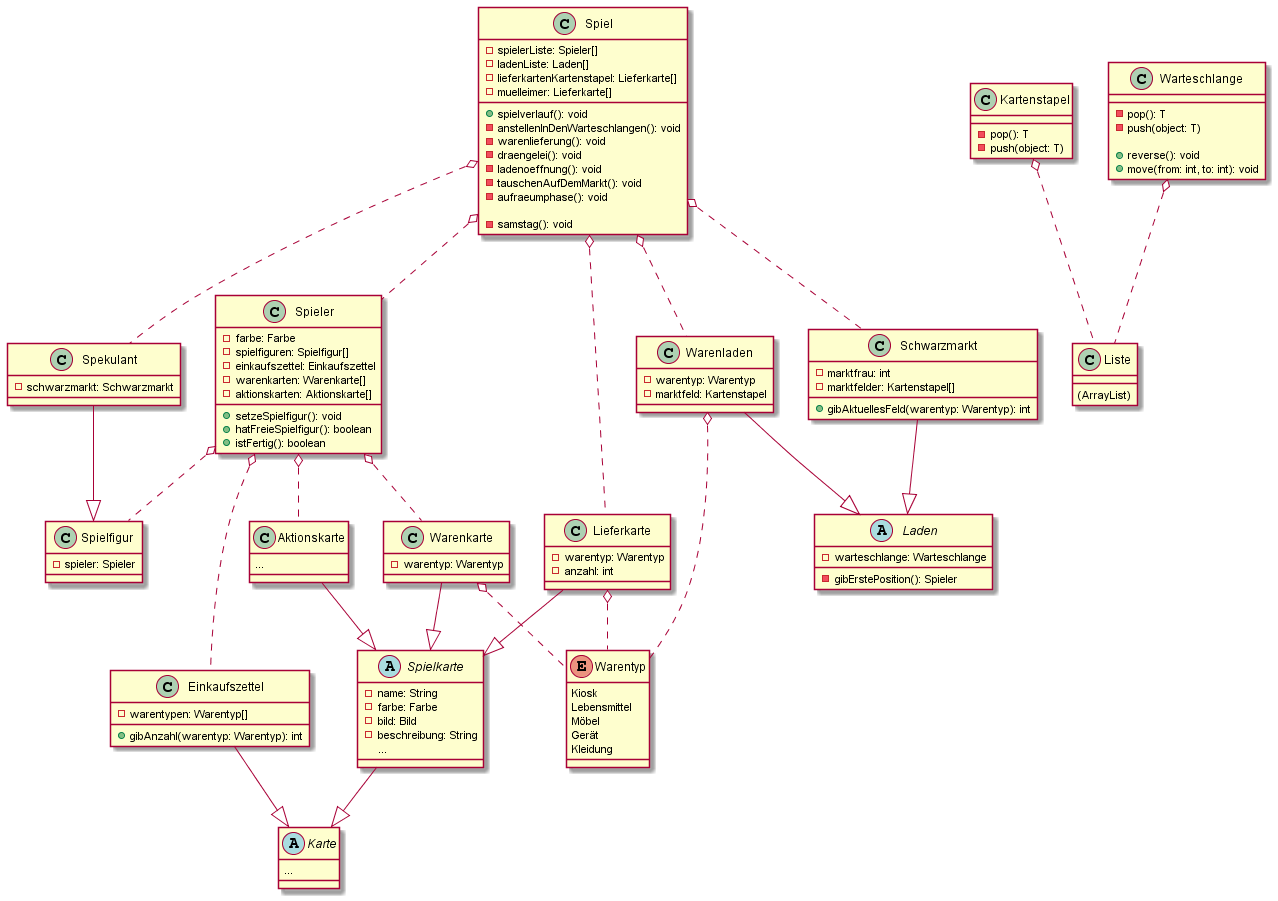
\includegraphics[height=0.85\textheight]{../../diagrams/out/architecture_overview/architecture_overview.png}
\end{frame}


\begin{frame}
	\frametitle{Klassenbeziehungen - Überblick - Umlet}
    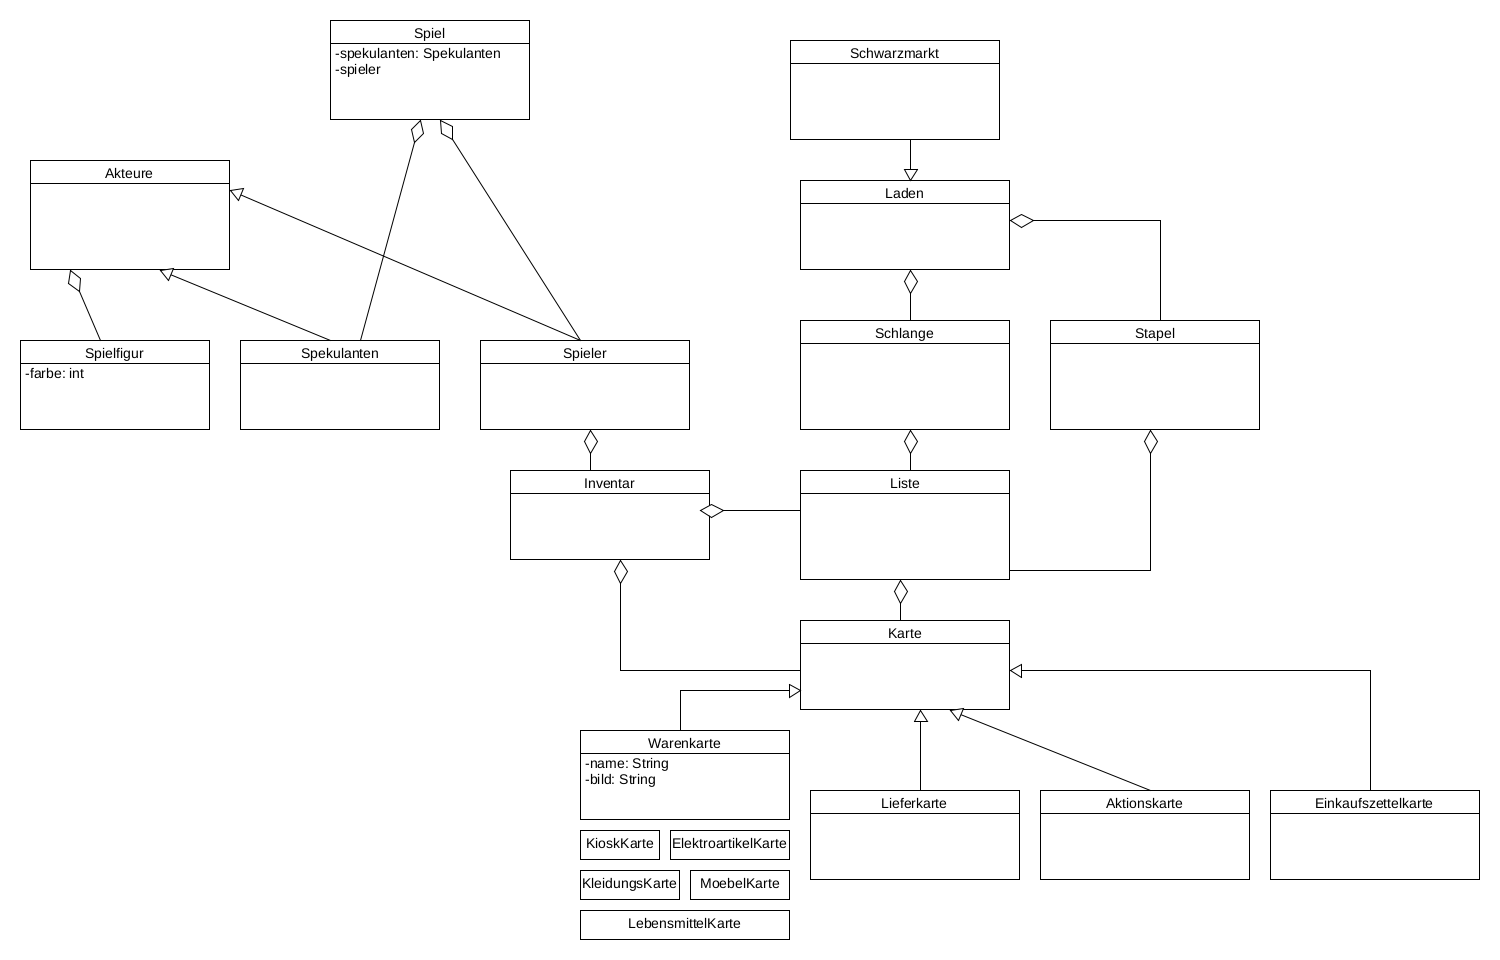
\includegraphics[height=0.8\textheight]{../../diagrams/out/umlet/kolejka_uml_26_04_2021.png}
\end{frame}


\begin{frame}
	\frametitle{Spiel}
	\begin{center}		
		\begin{tikzpicture}
			\umlclass{Spiel}{
				-spielerListe: Spieler[]\\
				-ladenListe: Laden[]\\
				-lieferkartenStapel: Lieferkarte[]\\
				-muelleimer: Lieferkarte[]\\
			}{
				+spielverlauf(): void\\
				-anstellenInDenWarteschlangen(): void\\
				-warenlieferung(): void\\
				-draengelei(): void\\
				-ladenoeffnung(): void\\
				-tauschenAufDemMarkt(): void\\
				-aufraeumphase(): void\\
				-samstag(): void\\
			}
		\end{tikzpicture}
	\end{center}
\end{frame}


\begin{frame}
	\frametitle{Spieler}	
		\begin{center}
			\begin{tikzpicture}
				\umlclass{Spieler}{
					-farbe: Farbe\\
					-spielfiguren: Spielfigur[]\\
					-einkaufszettel: Einkaufszettel\\
					-warenkarten: Warenkarte[]\\
					-aktionskarten: Aktionskarte[]\\
				}{
					+setzeSpielfigur(): void\\
					+hatFreieSpielfigur(): boolean\\
					+istFertig(): boolean\\
				}
			\end{tikzpicture}
		\end{center}
\end{frame}

\end{document}
